\documentclass[11pt,compress,t,notes=noshow, xcolor=table]{beamer}
\usepackage[]{graphicx}\usepackage[]{color}
% maxwidth is the original width if it is less than linewidth
% otherwise use linewidth (to make sure the graphics do not exceed the margin)
\makeatletter
\def\maxwidth{ %
  \ifdim\Gin@nat@width>\linewidth
    \linewidth
  \else
    \Gin@nat@width
  \fi
}
\makeatother

\newcommand{\citebutton}[2]{%
\beamergotobutton{\href{#2}{#1}}%
}

\newcommand{\blu}[1]{\textcolor{blue}{#1}}
\newcommand{\org}[1]{\textcolor{orange}{#1}}
\newcommand{\ques}{\textbf{\textcolor{red}{Question:  }}}
\newcommand{\questionssofar}{\begin{frame}\frametitle{Any questions?}\end{frame}}

\newcommand\warning{%
 \makebox[1.4em][c]{%
 \makebox[0pt][c]{\raisebox{.1em}{\scriptsize!}}%
 \makebox[0pt][c]{\color{red}\normalsize$\bigtriangleup$}}}%

\definecolor{fgcolor}{rgb}{0.345, 0.345, 0.345}
\newcommand{\hlnum}[1]{\textcolor[rgb]{0.686,0.059,0.569}{#1}}%
\newcommand{\hlstr}[1]{\textcolor[rgb]{0.192,0.494,0.8}{#1}}%
\newcommand{\hlcom}[1]{\textcolor[rgb]{0.678,0.584,0.686}{\textit{#1}}}%
\newcommand{\hlopt}[1]{\textcolor[rgb]{0,0,0}{#1}}%
\newcommand{\hlstd}[1]{\textcolor[rgb]{0.345,0.345,0.345}{#1}}%
\newcommand{\hlkwa}[1]{\textcolor[rgb]{0.161,0.373,0.58}{\textbf{#1}}}%
\newcommand{\hlkwb}[1]{\textcolor[rgb]{0.69,0.353,0.396}{#1}}%
\newcommand{\hlkwc}[1]{\textcolor[rgb]{0.333,0.667,0.333}{#1}}%
\newcommand{\hlkwd}[1]{\textcolor[rgb]{0.737,0.353,0.396}{\textbf{#1}}}%
\let\hlipl\hlkwb

\usepackage{framed}
\makeatletter
\newenvironment{kframe}{%
 \def\at@end@of@kframe{}%
 \ifinner\ifhmode%
  \def\at@end@of@kframe{\end{minipage}}%
  \begin{minipage}{\columnwidth}%
 \fi\fi%
 \def\FrameCommand##1{\hskip\@totalleftmargin \hskip-\fboxsep
 \colorbox{shadecolor}{##1}\hskip-\fboxsep
     % There is no \\@totalrightmargin, so:
     \hskip-\linewidth \hskip-\@totalleftmargin \hskip\columnwidth}%
 \MakeFramed {\advance\hsize-\width
   \@totalleftmargin\z@ \linewidth\hsize
   \@setminipage}}%
 {\par\unskip\endMakeFramed%
 \at@end@of@kframe}
\makeatother

\definecolor{shadecolor}{rgb}{.97, .97, .97}
\definecolor{messagecolor}{rgb}{0, 0, 0}
\definecolor{warningcolor}{rgb}{1, 0, 1}
\definecolor{errorcolor}{rgb}{1, 0, 0}
\newenvironment{knitrout}{}{} % an empty environment to be redefined in TeX

\usepackage{alltt}
\newcommand{\SweaveOpts}[1]{}  % do not interfere with LaTeX
\newcommand{\SweaveInput}[1]{} % because they are not real TeX commands
\newcommand{\Sexpr}[1]{}       % will only be parsed by R
\newcommand{\xmark}{\ding{55}}%


\usepackage[english]{babel}
\usepackage[utf8]{inputenc}

\usepackage{dsfont}
\usepackage{verbatim}
\usepackage{amsmath}
\usepackage{amsfonts}
\usepackage{amssymb}
\usepackage{bm}
\usepackage{csquotes}
\usepackage{multirow}
\usepackage{longtable}
\usepackage{booktabs}
\usepackage{enumerate}
\usepackage[absolute,overlay]{textpos}
\usepackage{psfrag}
\usepackage{algorithm}
\usepackage{algpseudocode}
\usepackage{eqnarray}
\usepackage{arydshln}
\usepackage{tabularx}
\usepackage{placeins}
\usepackage{tikz}
\usepackage{setspace}
\usepackage{colortbl}
\usepackage{mathtools}
\usepackage{wrapfig}
\usepackage{bm}
\usepackage{amsmath}
\usepackage{pifont}

\usetikzlibrary{shapes.multipart,shapes,arrows,automata,positioning,calc,chains,trees, shadows}
\tikzset{
  %Define standard arrow tip
  >=stealth',
  %Define style for boxes
  punkt/.style={
    rectangle,
    rounded corners,
    draw=black, very thick,
    text width=6.5em,
    minimum height=2em,
    text centered},
  % Define arrow style
  pil/.style={
    ->,
    thick,
    shorten <=2pt,
    shorten >=2pt,}
}

\tikzstyle{vec}=[draw, rectangle, fill = white, minimum width=5mm, minimum height=1cm, inner sep = 2pt]

\usepackage{subfig}

% Defines macros and environments
\usepackage{../../style/lmu-lecture}


\let\code=\texttt
\let\proglang=\textsf

\setkeys{Gin}{width=0.9\textwidth}

\setbeamertemplate{frametitle}{\expandafter\uppercase\expandafter\insertframetitle}

\usepackage{bbm}
% basic latex stuff
\newcommand{\pkg}[1]{{\fontseries{b}\selectfont #1}} %fontstyle for R packages
\newcommand{\lz}{\vspace{0.5cm}} %vertical space
\newcommand{\dlz}{\vspace{1cm}} %double vertical space
\newcommand{\oneliner}[1] % Oneliner for important statements
{\begin{block}{}\begin{center}\begin{Large}#1\end{Large}\end{center}\end{block}}


%new environments
\newenvironment{vbframe}  %frame with breaks and verbatim
{
 \begin{frame}[containsverbatim,allowframebreaks]
}
{
\end{frame}
}

\newenvironment{vframe}  %frame with verbatim without breaks (to avoid numbering one slided frames)
{
 \begin{frame}[containsverbatim]
}
{
\end{frame}
}

\newenvironment{blocki}[1]   % itemize block
{
 \begin{block}{#1}\begin{itemize}
}
{
\end{itemize}\end{block}
}

\newenvironment{fragileframe}[2]{  %fragile frame with framebreaks
\begin{frame}[allowframebreaks, fragile, environment = fragileframe]
\frametitle{#1}
#2}
{\end{frame}}


\newcommand{\myframe}[2]{  %short for frame with framebreaks
\begin{frame}[allowframebreaks]
\frametitle{#1}
#2
\end{frame}}

\newcommand{\remark}[1]{
  \textbf{Remark:} #1
}


\newenvironment{deleteframe}
{
\begingroup
\usebackgroundtemplate{
\includegraphics[width=\paperwidth,height=\paperheight]{../style/color/red.png}}
 \begin{frame}
}
{
\end{frame}
\endgroup
}
\newenvironment{simplifyframe}
{
\begingroup
\usebackgroundtemplate{
\includegraphics[width=\paperwidth,height=\paperheight]{../style/color/yellow.png}}
 \begin{frame}
}
{
\end{frame}
\endgroup
}\newenvironment{draftframe}
{
\begingroup
\usebackgroundtemplate{
\includegraphics[width=\paperwidth,height=\paperheight]{../style/color/green.jpg}}
 \begin{frame}
}
{
\end{frame}
\endgroup
}
% https://tex.stackexchange.com/a/261480: textcolor that works in mathmode
\makeatletter
\renewcommand*{\@textcolor}[3]{%
  \protect\leavevmode
  \begingroup
    \color#1{#2}#3%
  \endgroup
}
\makeatother





\input{../../latex-math/basic-math.tex}
\input{../../latex-math/basic-ml.tex}

%\newcommand{\titlefigure}{figure/gpt_sq.png}
\newcommand{\learninggoals}{
\item Understand Chinchilla
\item Understand the various scaling laws
}
\definecolor{texblue}{rgb}{0, 0, 1}
\def\myblue#1{\textcolor{texblue}{#1}}

\title{Training Large Language Models}
% \author{}
\institute{\href{https://slds-lmu.github.io/lecture_dl4nlp/}{slds-lmu.github.io/lecture\_dl4nlp}}
\date{}

\begin{document}
\lecturechapter{Scaling Laws and Chinchilla}
\lecture{Deep Learning for NLP}


%Notes:
% Slides: https://jasonwei20.github.io/files/FLAN%20talk%20external.pdf
% Check out emergence talk: https://www.youtube.com/watch?v=0SuyDLjNR9g

% LLM Survey: https://arxiv.org/pdf/2303.18223.pdf

% ------------------------------------------------------------------------------

\begin{vbframe}{Number of Parameters: Notation}

\vfill

\begin{itemize}
    \item Up to now in this chapter: number of parameters = $P$
    \item From now on: number of parameters = $N$
\end{itemize}

\vfill
    
\end{vbframe}

% ------------------------------------------------------------------------------

\begin{vbframe}{Scaling Laws}
\href{https://arxiv.org/abs/2001.08361}{\beamergotobutton{Kaplan et al. (2020)}} 

\vfill

\begin{itemize}

	\item Performance depends strongly on scale, weakly on model shape
	\begin{itemize}
	\item Scale means: parameters $N$, data $D$, and compute $C$
	\item Shape means: depth and width
	\end{itemize}

	\item Smooth power laws
	\begin{itemize}
	\item Performance has power-law relation with each factor $N$, $D$, $C$
	\item When not bottlenecked by the other two 
	\item Trend spanning more than six orders of magnitude
	\end{itemize}

	\item Universality of overfitting 
	\begin{itemize}
	\item Performance enters regime of diminishing returns if $N$ or $D$ held fixed while the other increases
	\end{itemize}

\end{itemize}

\vfill

\end{vbframe}

% ------------------------------------------------------------------------------

\begin{vbframe}{Scaling Laws}

\vfill

\begin{itemize}

	\item Universality of training
	\begin{itemize}
	\item Training curves follow predictable power-laws
	\item Their parameters are roughly independent of model size
	\item It is possible to predict by extrapolating the early part of the training curve
	\end{itemize}

	\item Transfer improves with test performance
	\begin{itemize}
	\item When evaluating on text with different distribution from training text, results are strongly correlated to those on the validation set
	\item Transfer to different distribution incurs a constant penalty but improves in line with performance on training set
	\end{itemize}

	\item Sample efficiency
	\begin{itemize}
	\item Large models are more sample-efficient than small models
	\item They reach same performance with fewer optimization steps
	\end{itemize}

\end{itemize}

\vfill

\end{vbframe}

% ------------------------------------------------------------------------------

\begin{vbframe}{Power Law (GPT3 Paper)}

\begin{figure}
    \centering
    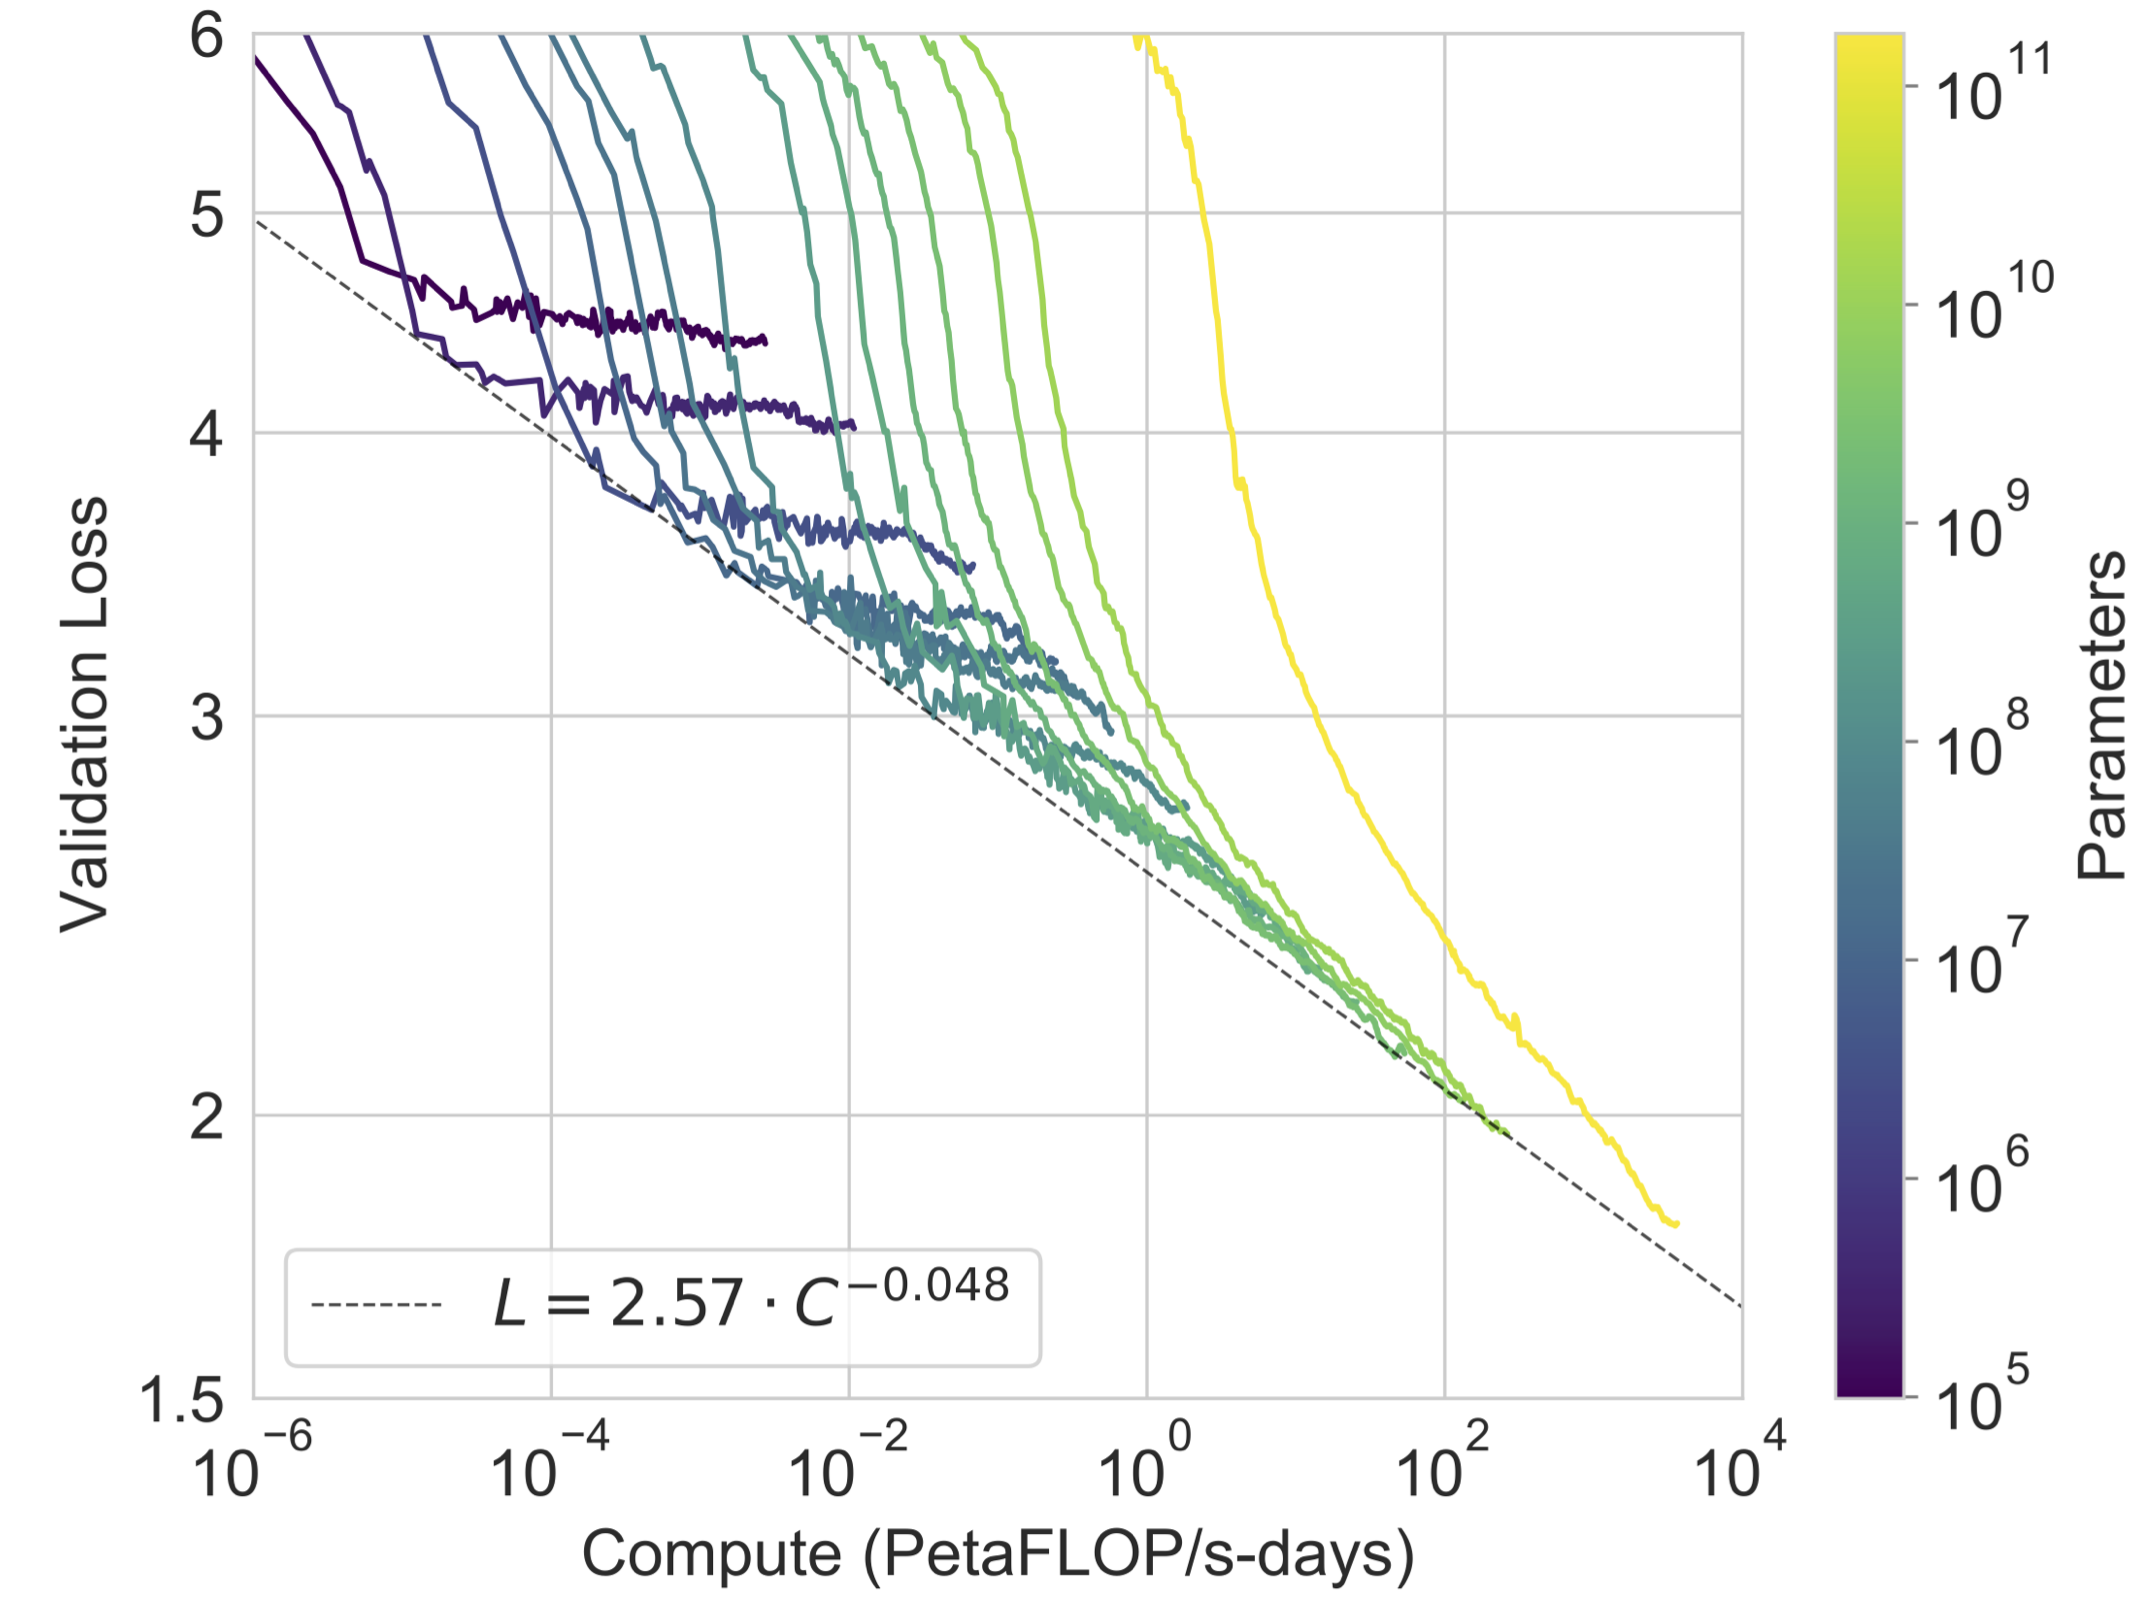
\includegraphics[width=10cm]{figure/losscompute.png}
\end{figure}
    
\end{vbframe}

% ------------------------------------------------------------------------------

\begin{vbframe}{Scaling Laws}

\vfill

\begin{itemize}

	\item Convergence is inefficient
	\begin{itemize}
	\item When $C$ is fixed but $N$ and $D$ are not, optimal performance is achived by training very large models and stopping significantly short of convergence  
	\end{itemize}

	\item Optimal batch size
	\begin{itemize}
    	\item “Optimal batch size: The ideal batch size for training these
                models is roughly a power of the loss only, and continues to
                be determinable by measuring the gradient noise scale
                [MKAT18]; it is roughly 1-2 million tokens at convergence for
                the largest models we can train.”
    	\item gradient noise scale = a measure of the signal-to-noise ratio
            of gradient across training examples
	\end{itemize}

\end{itemize}

\vskip3mm

\textbf{Larger language models will perform better and be more sample efficient than current models.} 

\vfill

\end{vbframe}

% ------------------------------------------------------------------------------

\begin{vbframe}{Optimal Batch Size}

\begin{figure}
    \centering
    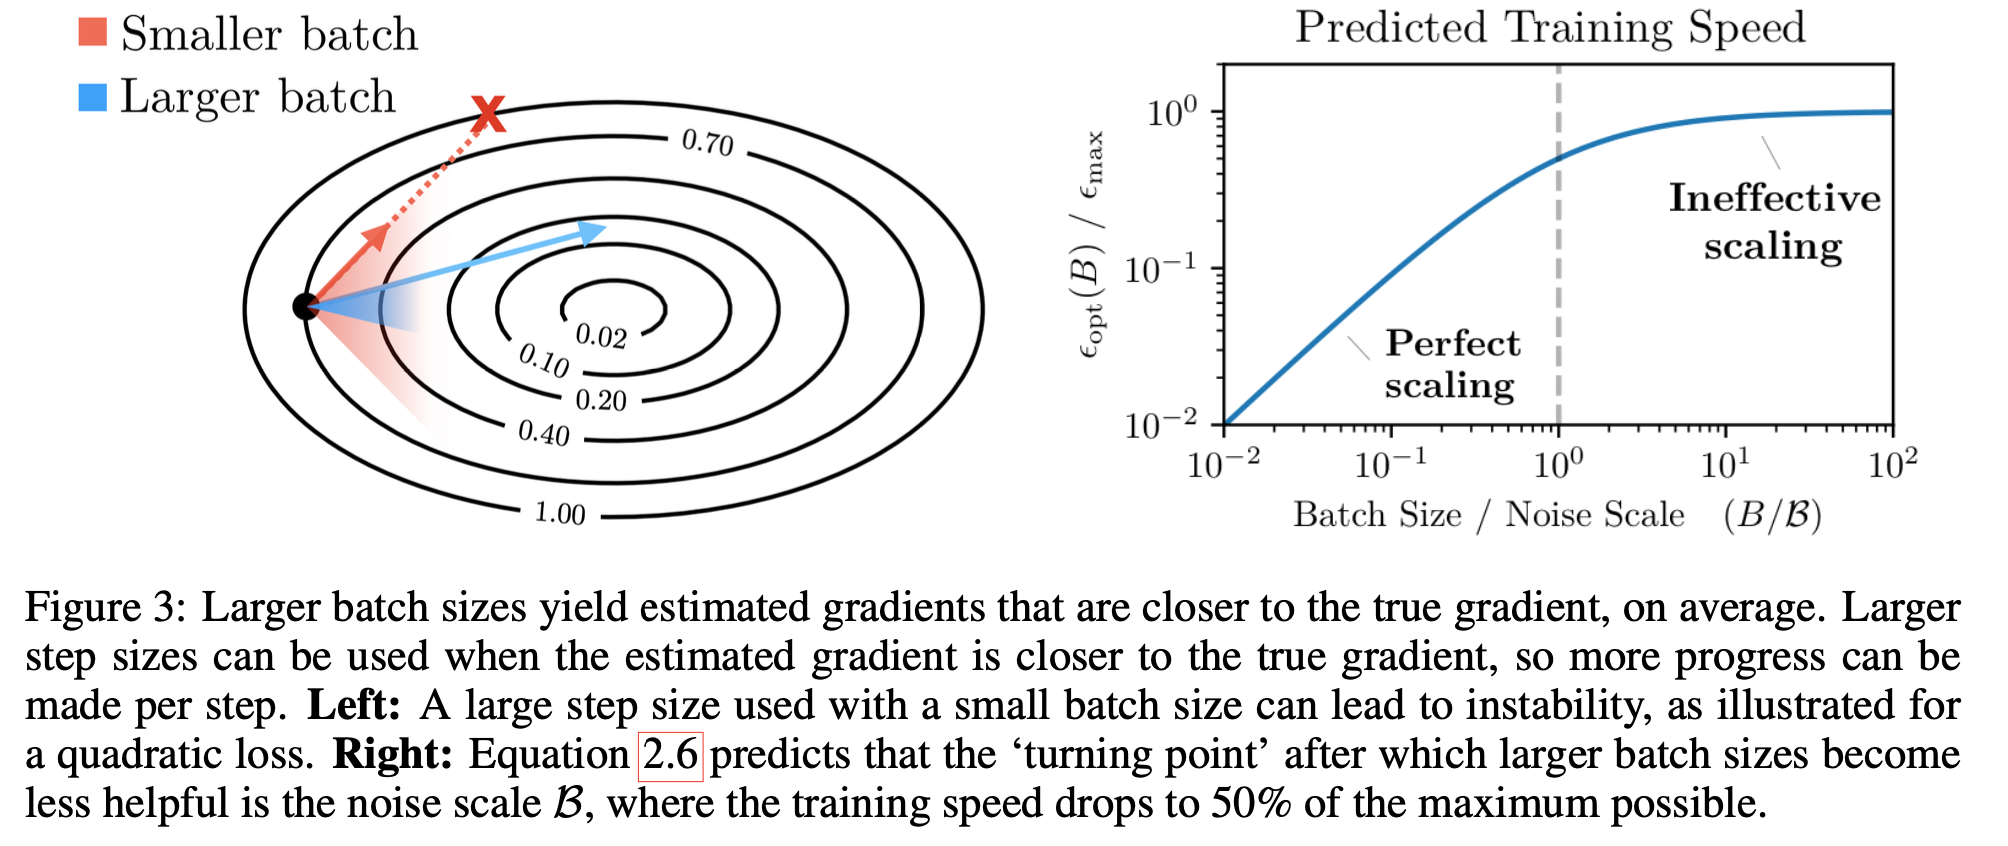
\includegraphics{figure/optimalbatchsize.png}
\end{figure}

\begin{itemize}
    \item Estimate gradient as accurately as possible $\rightarrow$ large batch
    \item Increase training speed as much as possible $\rightarrow$ large step size
    \item Based on the estimated gradient, choose a step size such that the cost of the landing position does not deviate too much from the cost of the ideal landing position $\rightarrow$ small step size
    \item Exploit stochasticity (epoch batches would not be a good thing even if we could compute them efficiently) $\rightarrow$ small step size

\end{itemize}

\end{vbframe}

% ------------------------------------------------------------------------------

\begin{vbframe}{Scaling Law for next word prediction}

\vfill

\begin{itemize}
    \item $L(N,D) = 1.61 + \frac{406.4}{N^{0.34}} + \frac{410.7}{D^{0.28}}$
    \item $L(N,D)$ is cross entropy on new text
\end{itemize}

\vfill

\end{vbframe}

% ------------------------------------------------------------------------------

\begin{vbframe}{Compute-Optimal LLM\MakeLowercase{s}}

Given a fixed FLOPs budget, how should we trade-off model size and text size to optimize performance? \citebutton{Hoffmann et al., 2022}{https://arxiv.org/abs/2203.15556}

\vfill

\begin{itemize}

	\item Find $N$ and $D$ so that $FLOPs(N,D) = C$ and $L(N,D)$ is minimal

	\item Empirically estimated $N$ and $D$ based on 400 models. 
	\begin{itemize}
	\item Ranging from 70\,M to 16\,B parameters
	\item Trained on 5\,B to 400\,B tokens
	\end{itemize}

	\item Different results from those of \citebutton{Kaplan et al., 2020}{https://arxiv.org/abs/2001.08361} 
	\item Results verified using Chinchilla
	\begin{itemize}
	\item Chinchilla has 70\,B parameters and is trained on 1.4\,T tokens
	\item 4x less parameters and 4x more tokens than Gopher
	\item Chinchilla outruns Gopher and has reduced memory footprint and inference cost 
	\end{itemize}

\end{itemize}

\vfill

\end{vbframe}

% ------------------------------------------------------------------------------

\begin{vbframe}{Compute-Optimal LLM\MakeLowercase{s}: Are GPT3 etc too large?}

\vfill

\begin{figure}
	\centering
	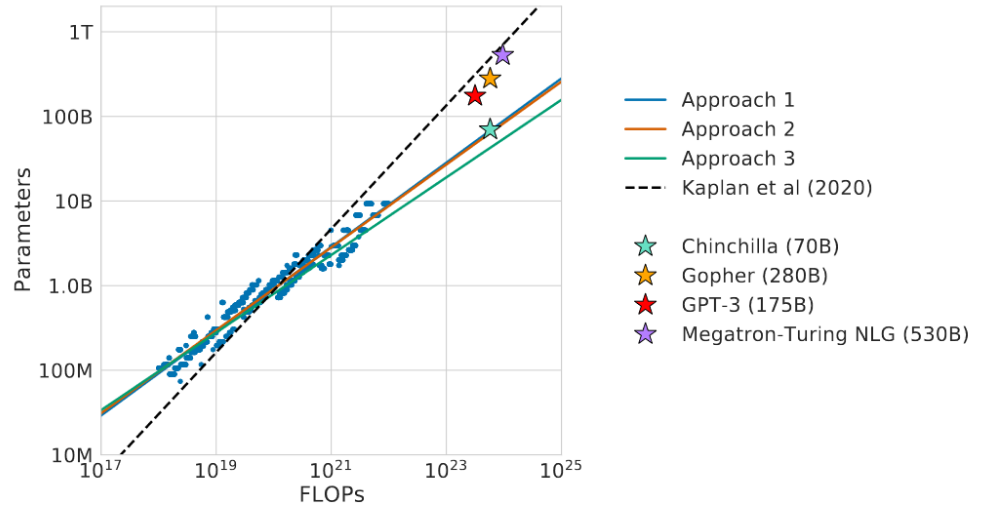
\includegraphics[width = 11cm]{./figure/chinchilla.png} \\ 
	\citebutton{Source: Hoffmann et al., 2022}{https://arxiv.org/abs/2203.15556}
\end{figure}

\vfill

\end{vbframe}

% ------------------------------------------------------------------------------

\begin{vbframe}{Compute-Optimal LLM\MakeLowercase{s} (2)}

Given a fixed FLOPs budget, how should one trade off model size and
the number of training tokens? We find that all three methods predict
that current large models should be substantially smaller and therefore
trained much longer than is currently done. Based on our estimated
compute-optimal frontier, we predict that for the compute budget used
to train Gopher, an optimal model should be 4 times smaller, while
being training on 4 times more tokens. We verify this by training a more
compute-optimal 70B model, called Chinchilla, on 1.4 trillion tokens.
Not only does Chinchilla outperform its much larger counterpart,
Gopher, but its reduced model size reduces inference cost considerably
and greatly facilitates downstream uses on smaller hardware. The
energy cost of a large language model is amortized through its usage
for inference and fine-tuning. The benefits of a more optimally trained
smaller model, therefore, extend beyond the immediate benefits of its
improved performance.

\end{vbframe}

% ------------------------------------------------------------------------------

\begin{vbframe}{Chinchilla and the other LLM\MakeLowercase{s}}

\vfill

\begin{figure}
	\centering
	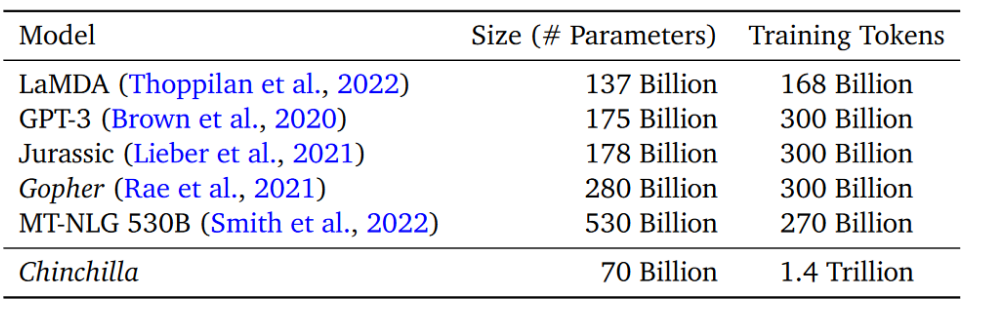
\includegraphics[width = 11cm]{./figure/llm_params.png} \\ 
	\citebutton{Source: Hoffmann et al., 2022}{https://arxiv.org/abs/2203.15556}
\end{figure}

\begin{figure}
	\centering
	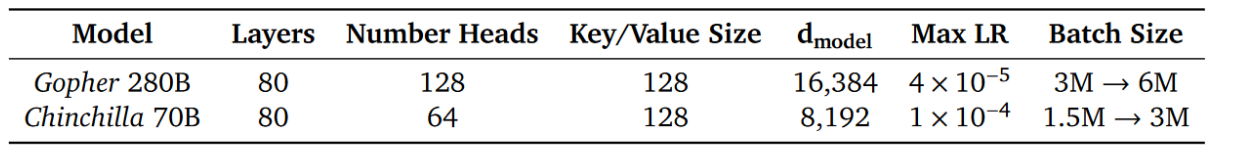
\includegraphics[width = 11cm]{./figure/chinchilla_gopher.png} \\ 
	\citebutton{Source: Hoffmann et al., 2022}{https://arxiv.org/abs/2203.15556}
\end{figure}

\vfill

\end{vbframe}

% ------------------------------------------------------------------------------

\begin{vbframe}{Chinchilla outperforms other LLM\MakeLowercase{s}: MMLU}

\vfill

\begin{figure}
	\centering
	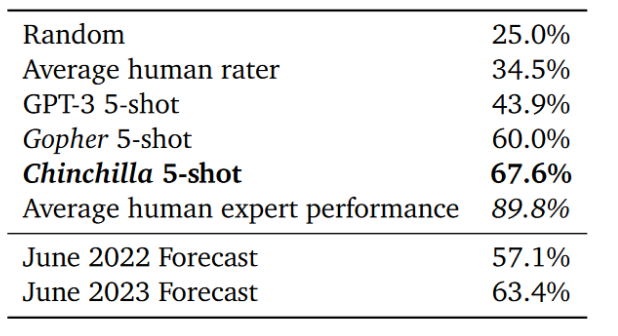
\includegraphics[width = 8cm]{./figure/chinchilla_mmlu.png} \\ 
	\citebutton{Source: Hoffmann et al., 2022}{https://arxiv.org/abs/2203.15556}
\end{figure}

\vfill

\end{vbframe}

% ------------------------------------------------------------------------------

\begin{vbframe}{Chinchilla outperforms other LLM\MakeLowercase{s}: QA}

\vfill

\begin{figure}
	\centering
	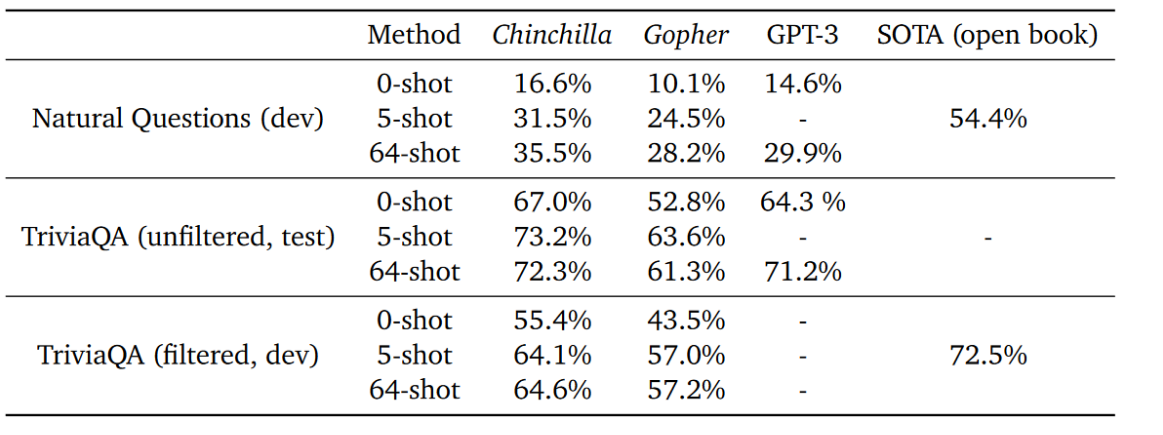
\includegraphics[width = 12cm]{./figure/chinchilla_qa.png} \\ 
	\citebutton{Source: Hoffmann et al., 2022}{https://arxiv.org/abs/2203.15556}
\end{figure}

\vfill

\end{vbframe}

% ------------------------------------------------------------------------------

\endlecture
\end{document}
